\section{Experiments}

\label{sec:experiments}

\subsection{Setup}

Experiments run on a single NVIDIA RTX 4090 (24\,GB) per run, four runs in parallel across four GPUs.
All results use the checkpoint with the highest validation accuracy, evaluated on the fixed 10{,}000-image test set.
Each trick is tested in isolation; the ``All methods'' condition applies all four simultaneously.

\subsection{Main Results}

\begin{table*}[ht]
    \centering
    \small
    \begin{tabular}{lrrrr}
        \toprule
        \multirow{2}{*}{Experiment}                            &
        \multicolumn{2}{c}{Weak recipe (100 ep, 61.68\% base)} &
        \multicolumn{2}{c}{Strong recipe (300 ep, 81.42\% base)}
        \\
        \cmidrule(lr){2-3}\cmidrule(lr){4-5}                   &
        Test Acc.                                              &
        $\Delta$                                               &
        Test Acc.                                              &
        $\Delta$
        \\
        \midrule
        Baseline                                               &
        61.68\%                                                &
        ---                                                    &
        81.42\%                                                &
        ---
        \\
        \midrule
        + \methodA{}                                           &
        \textbf{62.99\%}                                       &
        $+1.31$\pp{}                                           &
        77.03\%                                                &
        $-4.39$\pp{}
        \\
        + \methodD{}                                           &
        62.48\%                                                &
        $+0.80$\pp{}                                           &
        80.60\%                                                &
        $-0.82$\pp{}
        \\
        + \methodB{} (full, $\alpha{=}1.0$)                    &
        53.78\%                                                &
        $-7.90$\pp{}                                           &
        79.20\%                                                &
        $-2.22$\pp{}
        \\
        + \methodB{} (soft, $\alpha{=}0.3$)                    &
        60.52\%                                                &
        $-1.16$\pp{}                                           &
        \textbf{81.83\%}                                       &
        $+0.41$\pp{}
        \\
        + \methodC{}                                           &
        45.71\%                                                &
        $-15.97$\pp{}                                          &
        76.39\%                                                &
        $-5.03$\pp{}
        \\
        \midrule
        All methods                                            &
        38.05\%                                                &
        $-23.63$\pp{}                                          &
        71.74\%                                                &
        $-9.68$\pp{}
        \\
        \bottomrule
    \end{tabular}
    \caption{Test accuracy under both training recipes. $\Delta$ is relative to the corresponding baseline.
    Strong-recipe \methodC{} uses $s_i{=}1.0$ and cosine LR.
    Bold marks the best single-trick result per recipe.}
    \label{tab:results}
\end{table*}

Table~\ref{tab:results} shows the main results.
Under the \textbf{weak recipe}, whitening ($+1.31$\pp{}) and alternating flip ($+0.80$\pp{}) are net-positive; Dirac and ScaleBias+Lookahead are harmful ($-7.90$\pp{} and $-15.97$\pp{}); all methods combined yields the worst result ($-23.63$\pp{}).
Under the \textbf{strong recipe}, the ordering shifts: whitening flips to $-4.39$\pp{}, Dirac (full) narrows to $-2.22$\pp{}, and soft Dirac ($\alpha{=}0.3$) becomes the only net-positive trick ($+0.41$\pp{}).

\begin{table}[ht]
    \centering
    \setlength{\tabcolsep}{3pt}
    \small
    \begin{tabular}{rcccccc}
        \toprule
        Ep  & Base          & Alt           & White         & Dirac & SB+LA & All  \\
        \midrule
        50  & 47.8          & 49.7          & \textbf{53.4} & 41.2  & 40.2  & 44.8 \\
        100 & 61.6          & 60.9          & \textbf{60.5} & 53.4  & 53.3  & 55.7 \\
        150 & 68.2          & \textbf{69.3} & 65.2          & 63.6  & 63.2  & 61.2 \\
        200 & 71.9          & \textbf{73.8} & 68.8          & 69.6  & 67.8  & 65.3 \\
        250 & 75.7          & \textbf{77.3} & 73.8          & 74.7  & 71.5  & 68.3 \\
        300 & \textbf{81.1} & 81.0          & 77.0          & 79.2  & 75.3  & 70.8 \\
        \bottomrule
    \end{tabular}
    \caption{Validation accuracy (\%) at selected epochs, strong recipe.}
    \label{tab:epochs}
\end{table}

Table~\ref{tab:epochs} traces convergence under the strong recipe.
Whitening leads at epoch 50 (53.4\%) but is overtaken by epoch 150 as the frozen basis becomes mismatched to the increasingly augmented input distribution.

\begin{figure*}[ht]
    \centering
    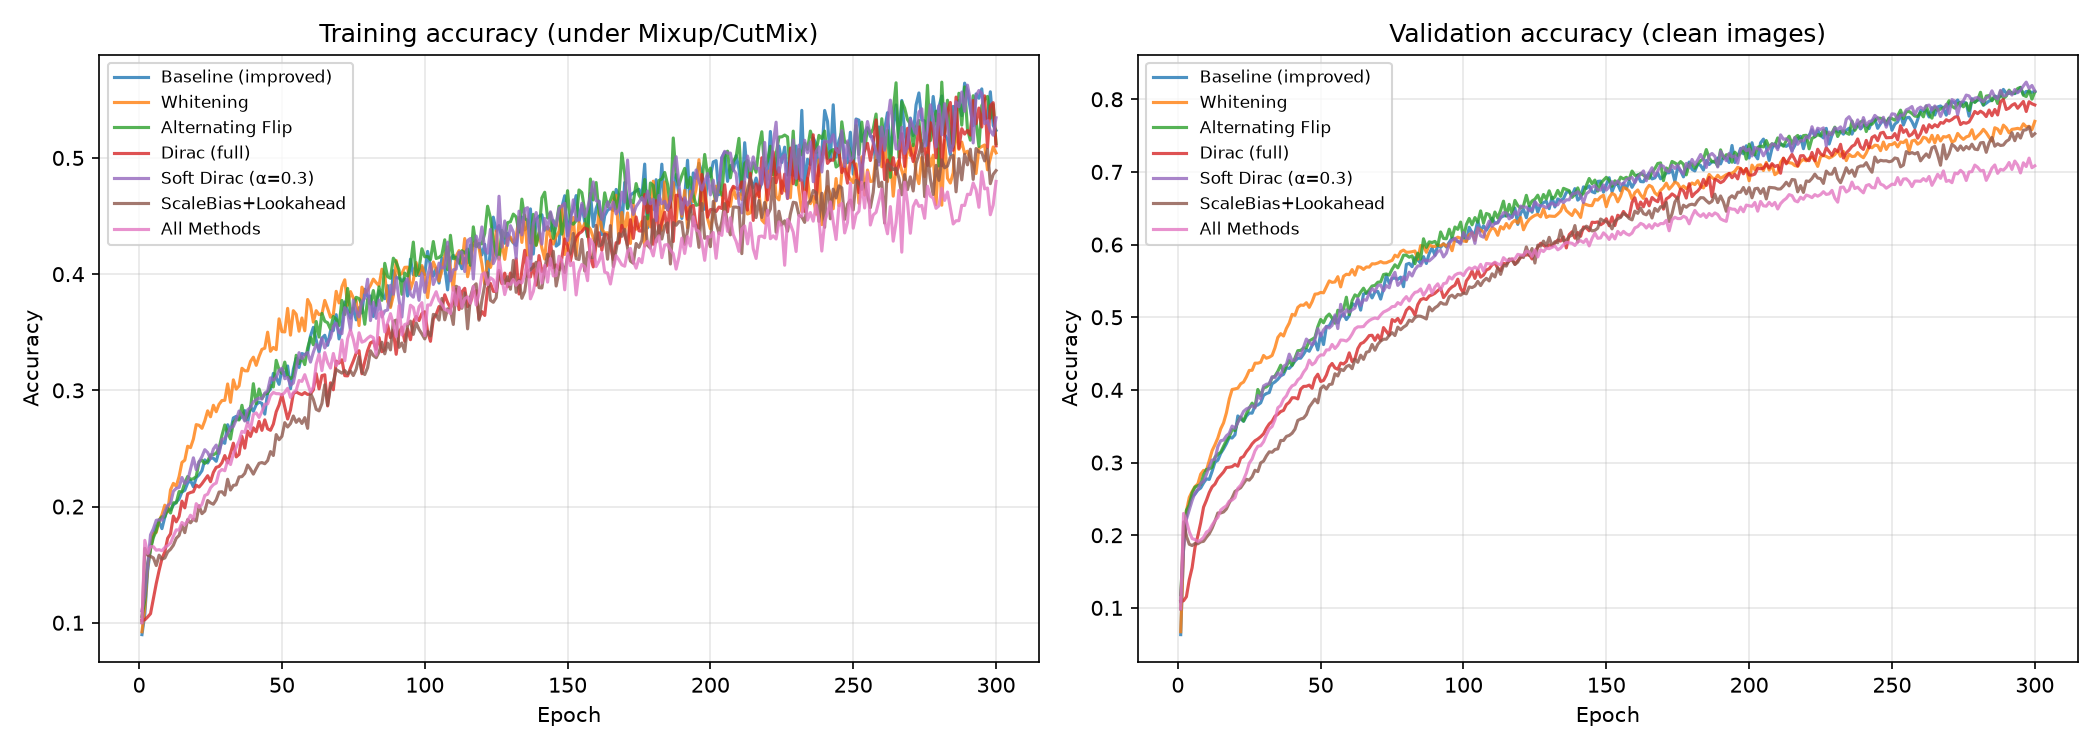
\includegraphics[width=\linewidth]{figures/comparison_v3.png}
    \caption{Validation accuracy over 300 epochs (strong recipe). Soft Dirac and Alternating Flip track the baseline; Whitening, ScaleBias+Lookahead, and All Methods fall behind.}
    \label{fig:curves}
\end{figure*}

\subsection{Why Whitening Reverses Under the Strong Recipe}

The whitened filters are eigenvectors of the patch covariance computed from \emph{clean} training images, then frozen.
Under the strong recipe, Mixup and CutMix blend pairs of images pixel-by-pixel, producing inputs whose patch statistics differ substantially from the clean-image basis.
Because the embedding is frozen, it cannot adapt.

\paragraph{CNN reconstruction confirms the mechanism.}
To isolate this effect, we run a controlled masked-pixel reconstruction experiment: a CNN encoder-decoder predicts the RGB values of 32 randomly masked $4\times4$ blocks per image, with \emph{no} augmentation beyond masking.

\begin{figure}[ht]
    \centering
    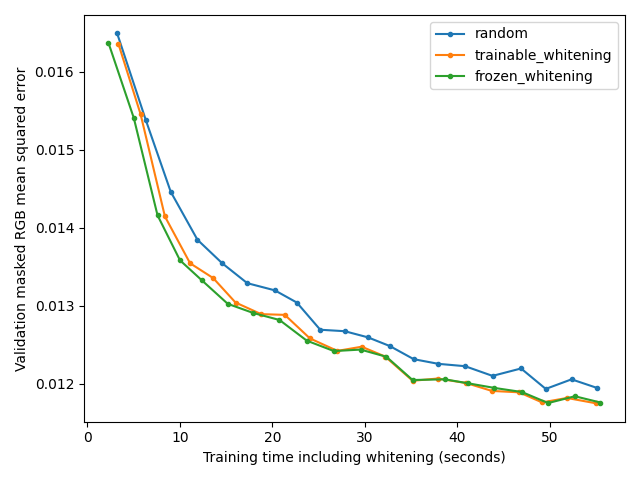
\includegraphics[width=\linewidth]{figures/cnn_reconstruction.png}
    \caption{Masked RGB reconstruction MSE over 20 epochs (lower is better). Both whitening variants beat the random baseline. Trainable and frozen whitening are nearly identical, confirming that freezing itself does not hurt---only the input-distribution mismatch does.}
    \label{fig:reconstruction}
\end{figure}

As Figure~\ref{fig:reconstruction} shows, both trainable and frozen whitening outperform the random baseline at every epoch (final MSE: 0.01175 / 0.01176 vs.\ 0.01195, $\sim$1.7\% relative improvement).
Critically, trainable and frozen whitening differ by only $\Delta = 0.000009$ MSE, confirming that \emph{freezing itself is not harmful}.
The reversal in the classification task therefore stems entirely from the mismatch between the frozen basis and the augmented inputs.

\subsection{All Tricks on CNN Reconstruction}

We extend the reconstruction study to test all four tricks individually and combined, using the same masked-RGB task with 20 epochs and no augmentation beyond masking.
Table~\ref{tab:recon} reports the final validation MSE, and Figure~\ref{fig:reconstruction_full} shows the convergence curves.

\begin{table}[ht]
    \centering
    \small
    \setlength{\tabcolsep}{4pt}
    \begin{tabular}{lrr}
        \toprule
        Variant           & Val MSE (ep 20) & $\Delta$ vs baseline \\
        \midrule
        Baseline          & 0.012207 & ---           \\
        \midrule
        Frozen whitening  & 0.012042 & $-$1.35\%     \\
        Alternating flip  & 0.012116 & $-$0.75\%     \\
        ScaleBias         & 0.012016 & $-$1.56\%     \\
        Dirac init        & 0.011982 & $-$1.84\%     \\
        Lookahead         & \underline{0.011581} & $-$5.12\% \\
        \midrule
        All methods       & \textbf{0.011075} & $-$9.27\% \\
        \bottomrule
    \end{tabular}
    \caption{Final validation MSE on masked RGB reconstruction (lower is better).
        $\Delta$ is relative improvement over the baseline MSE.}
    \label{tab:recon}
\end{table}

\begin{figure}[ht]
    \centering
    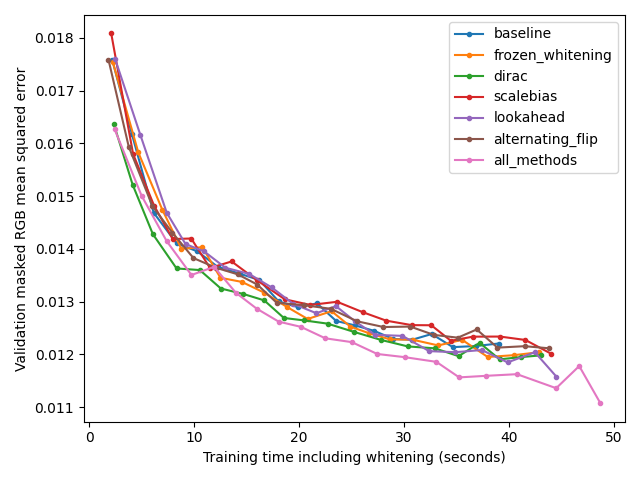
\includegraphics[width=\linewidth]{figures/cnn_reconstruction_full.png}
    \caption{MSE convergence over 20 epochs for all trick variants on CNN masked reconstruction.
        All tricks improve over the baseline; Lookahead is the strongest single trick, and all methods combined achieves the best result.}
    \label{fig:reconstruction_full}
\end{figure}

The results tell a strikingly different story from the ViT classification experiments.
\emph{All} tricks reduce validation MSE, every single trick is helpful, and they compose constructively: all methods combined achieves $-9.27\%$ relative improvement, the best result.

Three observations explain why reconstruction behaves differently from classification.

\textbf{(1) Frozen whitening works because there is no augmentation conflict.}
Masking preserves the patch covariance of the original images, so the frozen whitened basis remains matched to the actual inputs throughout training.
The $-1.35\%$ improvement mirrors the weak-recipe ViT result ($+1.31$\pp{}) and directly confirms that the reversal under the strong recipe was caused by augmentation mismatch, not by freezing.

\textbf{(2) Lookahead is the strongest single trick ($-5.12\%$).}
In the ViT experiments, Lookahead conflicted with the cyclic LR schedule.
Here, we use a flat Adam LR for the reconstruction model---the regime for which Lookahead was originally validated.
Without the schedule conflict, its slow-weight stabilisation reduces oscillation and produces smooth, monotonic convergence.
This directly validates our diagnosis from the ViT experiments: Lookahead's harmful interaction was with the decaying LR schedule, not with learning in general.

\textbf{(3) Dirac init helps in a CNN reconstruction model.}
Unlike in the ViT, where Dirac init collapses self-attention heads into a uniform transformation, the CNN's grouped convolutions are not subject to the same symmetry pathology.
Near-identity initialisation allows early layers to act as pass-throughs while the decoder learns to predict masked regions, and specialisation emerges gradually.
The $-1.84\%$ improvement is consistent with its intended behaviour in the original paper.

Together, these results complete the transferability picture.
When tricks are tested on the architecture and task they were designed for (or on a task that avoids their known failure modes), they are uniformly effective and compose well.
The failures observed in ViT classification are not intrinsic to the tricks themselves but arise from specific mismatches: frozen whitening with strong augmentation, Dirac init with attention symmetry, and Lookahead with decaying LR schedules.

\subsection{Why Dirac Init Improves With Strong Augmentation}

Full identity initialisation collapses all attention heads to the same transformation at epoch 0:
\begin{equation}
    \operatorname{Attn}(X) =
    \operatorname{softmax} \!\left(
    \frac{XX^\transpose}{\sqrt{d}}
    \right) X.
\end{equation}
The model must break this symmetry before specialising, wasting early training.
Under the weak recipe this costs $-7.90$\pp{}; under the strong recipe Mixup/CutMix supply the gradient diversity needed to break symmetry faster, narrowing the gap to $-2.22$\pp{}.
Soft Dirac ($\alpha=0.3$) avoids the full collapse while retaining a mild identity prior, turning net-positive under the strong recipe ($+0.41$\pp{}).

\subsection{Why ScaleBias + Lookahead Hurts}

Two independent issues compound.
First, initialising ScaleBias with $s_i{=}1/9$ suppresses gradients reaching the transformer body by $0.11\times$; fixing to $s_i{=}1.0$ removes this.
Second, Lookahead's slow-weight pull ($\phi\gets\phi+\alpha(\theta-\phi)$, $\theta\gets\phi$) partially reverses fast-weight progress every $k$ steps.
Under a flat LR the fast weights converge in a consistent direction, so the pull is benign.
Under OneCycleLR or cosine decay, the direction changes substantially across $k$ steps, introducing conflicting gradient history.
The residual $-5.03$\pp{} after both fixes suggests that only a flat LR fully decouples Lookahead from the schedule.

\subsection{Discussion}

The results reveal two orthogonal axes of compatibility:
\begin{enumerate}[leftmargin=*,topsep=2pt,itemsep=1pt]
    \item \textbf{Architectural:} Dirac init and post-pooling output scaling assume convolutional structure and remain net-negative in transformers (though gaps narrow with appropriate fixes).
    \item \textbf{Recipe:} Frozen whitening and Lookahead depend on training-recipe properties (augmentation statistics, LR schedule shape) independently of architecture.
\end{enumerate}
The ``All methods combined'' condition is the worst result under both recipes, confirming that the failure modes are additive rather than self-cancelling.
